\documentclass[]{antposter}

% Poster metadata
\title{Better Poster}
\subtitle{Evidence-based Design}
\author{David Woodburn, Ph.D.}
\secondauthor{Mike Morrison, Ph.D.}
\thirdauthor{Lt Col Michael Faraday}
\fourthauthor{Maj Carl F. Gauss}
% Multiple lines must be separated by '\?'.
\qrdata{https://youtu.be/SYk29tnxASs?si=drWywhECG4VRmiCW}
\abstract{
    \textbf{Main finding} goes here, translated into \textbf{plain
    English}. \textbf{Emphasize} the important words.

    % Graphic
    \vspace{2.0cm}\normalsize\centering
    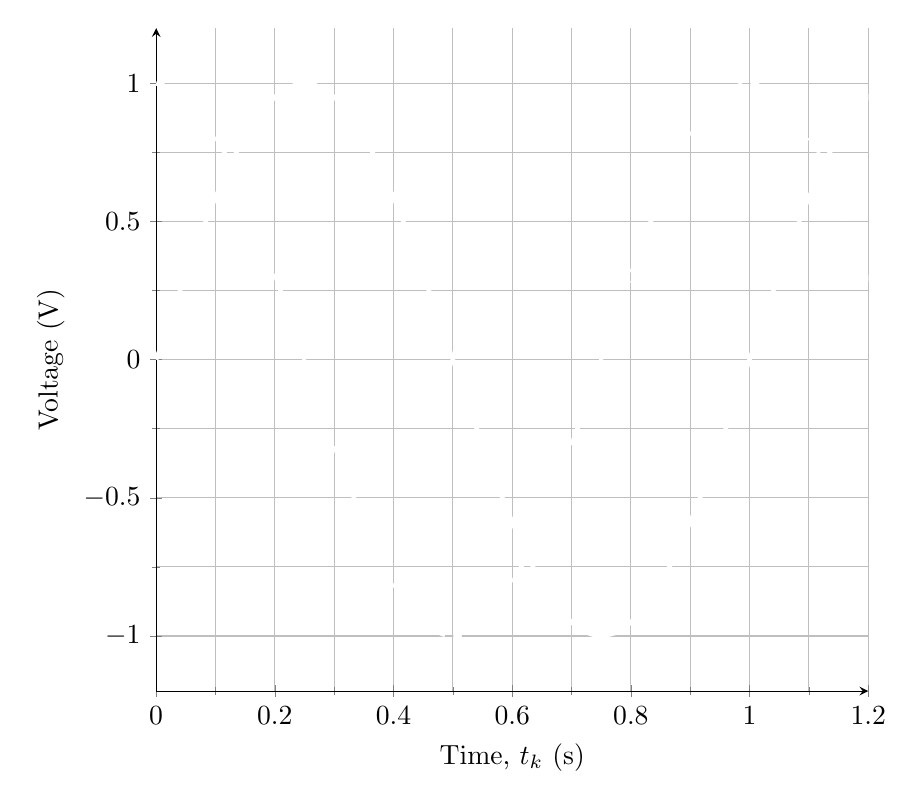
\begin{tikzpicture}
        \newlength{\Width}\setlength{\Width}{\textwidth}
        \addtolength{\Width}{-1.5cm}
        \begin{axis}[
                width=\Width, height=10cm,
                axis lines=left, grid=both,
                xmax=1.2, enlarge y limits=true,
                minor tick num=1,
                xlabel={Time, $t_k$ (s)},
                ylabel={Voltage (V)}]
            \addplot[ultra thick, white, domain=0:2, samples=120]
                {sin(360*\x)};
            \addplot[ultra thick, white, dashed, domain=0:2, samples=120]
                {cos(360*\x)};
        \end{axis}
    \end{tikzpicture}
}

\begin{document}
\maketitle

\section{Background}

Dr. Mike Morrison's research on poster design psychology has led to widely
adopted layouts, with over 250\,000 downloads of his PowerPoint
version\footnote{\url{https://osf.io/6ua4k}}. This template offers a \LaTeX{}
alternative.

\section{Method}

\subsection{Central Abstract}

The main finding of your research is highlighted in large text on a dark
background to capture the reader's attention first. This key result, along with
any striking figures, is entered as the abstract using the \verb|\abstract{}|
macro.

\subsection{Multiple Authors}

You can include up to four authors with this class:
\begin{center}
\begin{tabular}{l|l}
    \verb|\author{}|       & \verb|\thirdauthor{}| \\
    \verb|\secondauthor{}| & \verb|\fourthauthor{}|
\end{tabular}
\end{center}

\subsection{Built-in QR Codes}

You can include a QR code in your poster using the \verb|\qrdata{}| command.
While it may not be suitable for all cases (e.g., CUI or classified content), it
is useful in many situations. Simply input the URL into the \verb|qrdata|
command, and a QR code will be generated automatically---no need for external
tools or adjustments.

\subsection{Color Themes}

The \verb|antposter| class takes any one of the following color options to set
the background color of the center abstract area (default \verb|azure|):
\begin{center}
    \begin{tabular}{l|l|l|l|l}
        \texttt{blue}  & \texttt{cyan}  & \texttt{lime}
            & \texttt{red}    & \texttt{magenta} \\
        \texttt{azure} & \texttt{green} & \texttt{yellow}
            & \texttt{orange} & \texttt{purple}
    \end{tabular}
\end{center}

\subsection{Logos}

By default, the ANT Center and AFIT logos are displayed. If you only want the
ANT Center compass, use the \verb|compassonly| class option. For the AFIT logo
alone, use \verb|afit|. If you want to use a custom logo, use the \verb|\logo{}|
command.

\logo{../presentation-files/cornell}

\subsection{Layouts}

There are two layouts: three-part (default) and two-part. To switch to two-part,
use the \verb|twopart| option in the document class.


\begin{tabular}{@{}c@{}}
    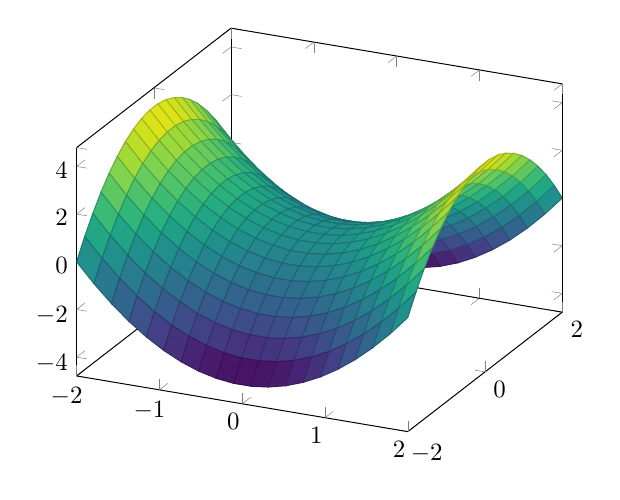
\begin{tikzpicture}[scale=0.9]
        \pgfplotsset{colormap/viridis}
        \begin{axis}[samples=20]
            \addplot3[surf, domain=-2:2] {x^2-y^2};
        \end{axis}
    \end{tikzpicture} \\
    The Pringle's surface.
\end{tabular}

% Macro to plot bars in polar coordinates
\vfill
\newcommand{\polarbar}[3]{
    \pgfmathsetmacro{\x}{#1*cos(#2)}
    \pgfmathsetmacro{\y}{#1*sin(#2)}
    \draw[fill=blue!50] (0,0) -- (\x,\y) arc[start angle=#2,
        end angle=#2+#3, radius=#1] -- cycle;
}
\begin{tabular}{@{}c@{}}
    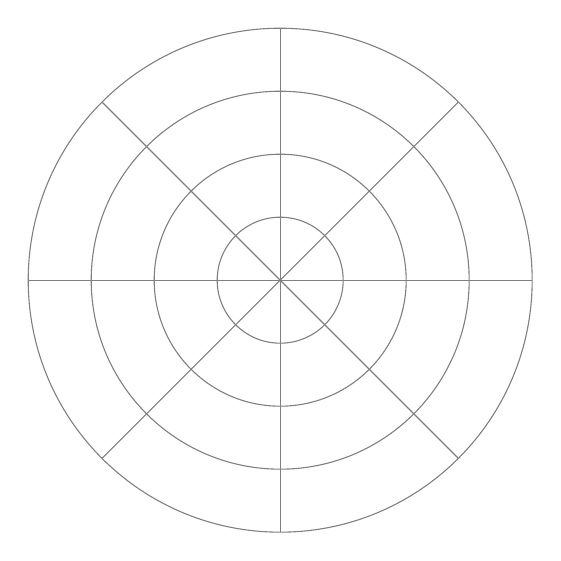
\begin{tikzpicture}[scale=0.8]
        % Draw polar bars (radius, angle, angle span)
        \polarbar{3}{0}{45}
        \polarbar{1}{45}{45}
        \polarbar{2}{90}{45}
        \polarbar{5}{135}{45}
        \polarbar{3}{180}{45}
        \polarbar{4}{225}{45}
        \polarbar{2}{270}{45}
        \polarbar{1}{315}{45}
        
        % Draw polar grid
        \draw[gray, thin] (0,0) circle(4); % Max radius circle
        \draw[gray, thin] (0,0) circle(3); % Intermediate radius circle
        \draw[gray, thin] (0,0) circle(2); % Small radius circle
        \draw[gray, thin] (0,0) circle(1); % Smallest radius circle
        \foreach \angle in {0,45,...,315} {
            \draw[gray, thin] (0,0) -- (\angle:4); % Radial lines
        }
    \end{tikzpicture} \\
    Polar plot example.
\end{tabular}

\vfill
\begin{tabular}{@{}c@{}}
    \begin{tikzpicture}[scale=0.8]
        \path (-4,0) -- (5,0);
        \foreach \p/\C [count=\n] in {50/lime, 43/azure, 36/orange,
                29/purple, 17/red} {
            \pgfmathsetmacro{\ang}{3.6*\p}
            \pgfmathsetmacro{\rad}{1.0*\n}
            \draw[\C, line width=10pt] (\rad,0) arc (0:\ang:\rad)
                node[anchor={\ang-90}, inner sep=0pt]{\p\%};
        }
    \end{tikzpicture} \\
    Polar bar graph example.
\end{tabular}

\end{document}
